\subsection{最优间隔分类器-优化方法}
\begin{enumerate}
	\item 根据前面推导出来的优化目标及拉格朗日对偶规划的内容,我们可以得到不等式约束为:
	\begin{align}
		g_i(w) = -y^{(i)}\left(w^Tx^{(i)}+b\right)+1 \leq 0
	\end{align}
	在此问题中,没有等式约束。\\
	由前面提到的KKT对偶互补条件可知,当且仅当$g_i(w)=0$时,$\alpha_i$可以不为0。令$g_i(w)=0$的点就是几何间隔$=1$的点,即与决策边界最靠近的点\footnote{在我们前面的推导过程中,有让几何间隔$=1$,所以这些点就是离决策边界最近的点},这些点称为支撑向量(Support Vectors),如下图3个红框标识的点:
	\begin{figure}[htbp]
		\centering
		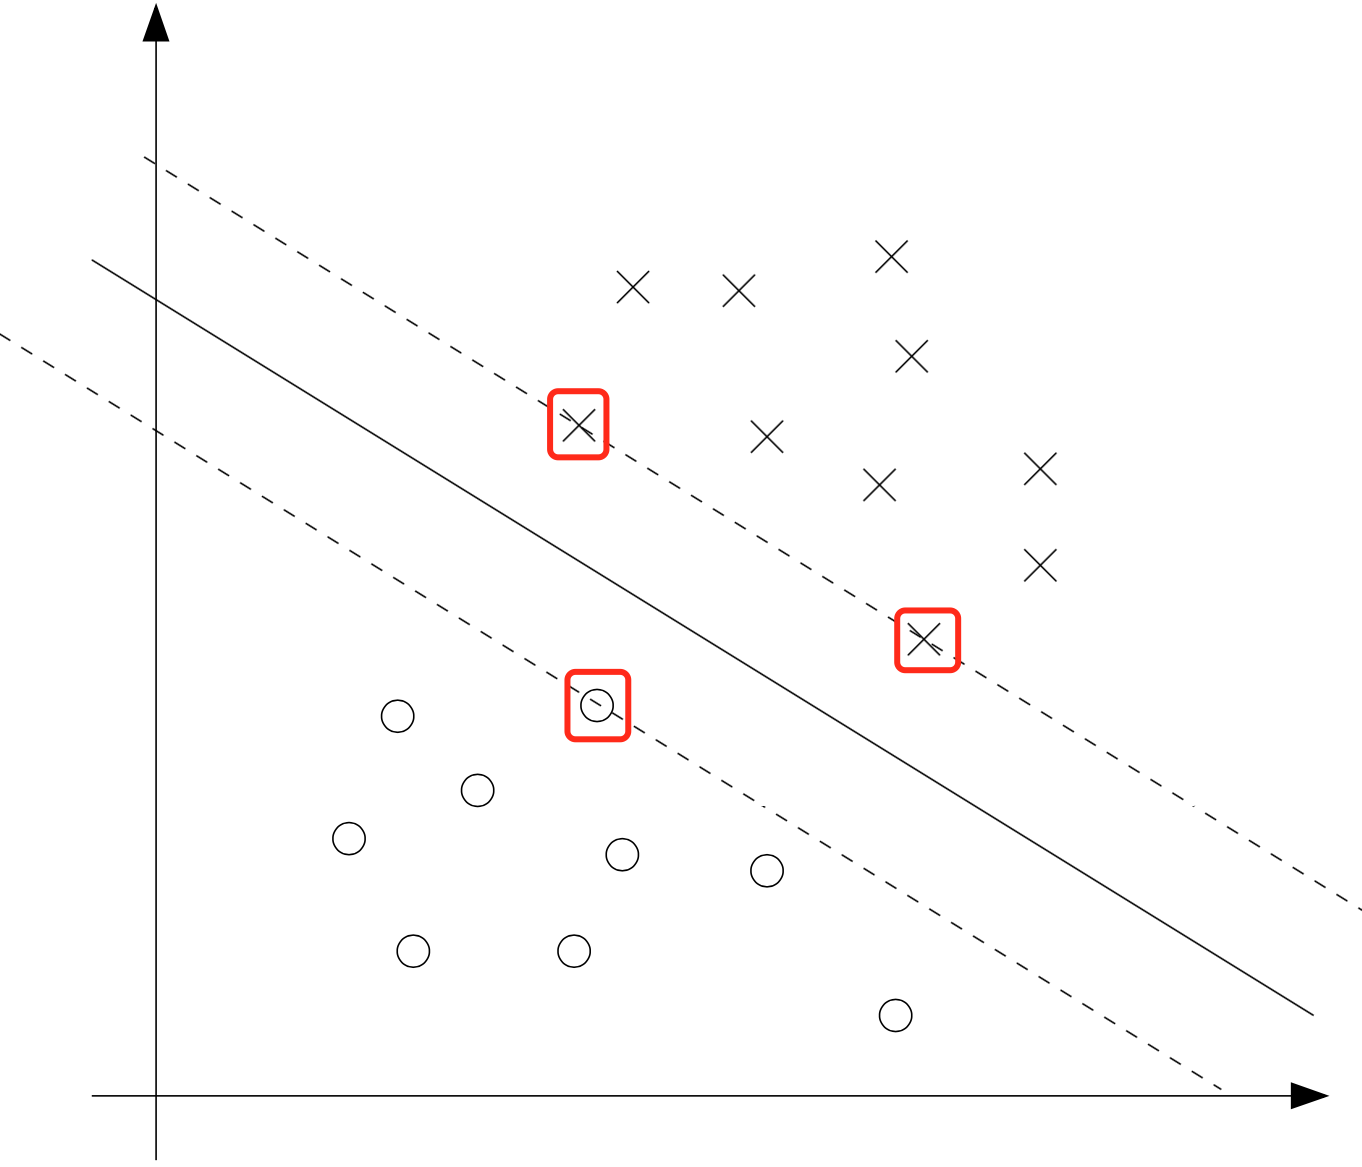
\includegraphics[scale=0.35]{images/支撑向量}
		\caption{支撑向量}
	\end{figure}

	\item 拉格朗日函数为:
	\begin{align}
		\mathcal{L}(w, b, \alpha) = \frac{1}{2}\|w\|^2 - \sum_{i=1}^{m}\alpha_i \left[y^{(i)}(w^Tx^{(i)}+b)-1\right]
	\end{align}
	注意,因为在我们的问题中没有等式约束,故上式没有$\beta_i$。

	\item 接下来我们对拉格朗日函数求偏导数,令偏导数的值为0。
	\begin{align}
		\nabla_{w}\mathcal{L}(w,b,\alpha)=w - \sum_{i=1}^{m}\alpha_iy^{(i)}x^{(i)}=0
	\end{align}
	可得:
	\begin{align}
		w = \sum_{i=1}^{m}\alpha_iy^{(i)}x^{(i)}
		\label{$w$}
	\end{align}
	对$b$:
	\begin{align}
		\frac{\partial}{\partial b}\mathcal{L}(w,b,a) = \sum_{i=1}^{m}a_iy^{(i)}=0
		\label{b}
	\end{align}
	将\ref{$w$}代入拉格朗日函数,得:
	\begin{align}
		\mathcal{L}(w,b,\alpha) = \sum_{i=1}^{m}\alpha_i-\frac{1}{2}\sum_{i,j=1}^{m}y^{(i)}y^{(j)}\alpha_i\alpha_j (x^{(i)})^Tx^{(j)} - b\sum_{i=1}^{m}a_iy^{(i)}
	\end{align}
	再将\ref{b}代入上式,得到:
	\begin{align}
		\mathcal{L}(w,b,\alpha) = \sum_{i=1}^{m}\alpha_i-\frac{1}{2}\sum_{i,j=1}^{m}y^{(i)}y^{(j)}\alpha_i\alpha_j (x^{(i)})^Tx^{(j)}
	\end{align}
	\item 下面我们考虑原问题的对偶优化问题,即:
	\begin{align}
		&\text{优化目标:} \\
		& \qquad \max_{\alpha} W(\alpha) = \sum_{i=1}^{m}\alpha_i-\frac{1}{2}\sum_{i,j=1}^{m}y^{(i)}y^{(j)}\alpha_i\alpha_j \langle x^{(i)}, x^{(j)}\rangle \\
		&\text{约束条件:} \\
		& \qquad \alpha_i \geq 0, \quad i=1,\dots,m \\
		& \qquad \sum_{i=1}^{m}\alpha_iy^{(i)} = 0
	\end{align}
	其中,$\langle x^{(i)}, x^{(j)}\rangle $表示内积\\
	第一个约束是我们一直有的,第二个约束通过求$b$的偏导数后得到\footnote{吴恩达在视频中解释这个约束说明的意义:若$\sum_{i=1}^{m}\alpha_iy^{(i)} \neq 0$,则$\theta_{\mathcal{D}}(\alpha)=-\infty$,所以,如果我们要$\max \theta_{\mathcal{D}}(\alpha)$,就应该取那些能让$\sum_{i=1}^{m}\alpha_iy^{(i)} = 0$的$\alpha$,这样,$\theta_{\mathcal{D}}(\alpha)=W(\alpha)$。{\color{red}{我也没怎么懂,待后面研究研究}}}。

	\item 若要得到$w$,根据公式\ref{$w$},我们可以知道,只要求得了$\alpha$就能得到$w$

	\item 在开始计算前,我们再仔细看下公式\ref{$w$},$w$是关于$\alpha$的函数,我们将其代入$w^Tx+b$后可以发现:
	\begin{align}
		w^Tx + b &= \left( \sum_{i=1}^{m}\alpha_i y^{(i)}x^{(i)} \right)^Tx + b \\
		&= \sum_{i=1}^{m}\alpha_iy^{(i)}\langle x^{(i)}, x \rangle + b \\
		&\downarrow	\\
		h_{w,b}(x) &= g(w^Tx + b) \\
		&= g(\sum_{i=1}^{m}\alpha_iy^{(i)}\langle x^{(i)}, x \rangle + b)
	\end{align}
	前面我们已经讨论过了,除了支撑向量对应的那几个点之外,其余的点$\alpha_i$均为0,而支撑向量的数目很少,这将大大简化我们的计算。

	\item 假设我们已经得到了$w^*$,我们便得到了一堆的平行线(因为决策边界只剩截距$b$不知道了),我们自然会取两类点中间的直线,这样才能保证离每一类都最远,于是:
	\begin{align}
		b^* = - \frac{\max_{i;y^{(i)}=-1}w^*x^{(i)} + \max_{i;y^{(i)}=1}w^*x^{(i)}}{2}
	\end{align}


\end{enumerate}

















